\section{Conceptual design options} \label{ch:options}
This chapter will discuss the five design concepts that will be considered in this report. First the selection of concepts based on the shape, mission duration and controls system design option trees is made. For the six configurations of the \gls{br} one is disregarded as it has no additional advantages over the other concepts. In section \ref{sec:conf} the five selected configurations are sketched and described. A simple load analysis is given in the form of \gls{fbd} to gain insight in the functioning of each of the concepts. The following five design are consequently used for analysis in the relevant chapters of this report. Finally the control systems corresponding to the each of the shape configurations are discussed in chapter \ref{sec:ccs}. A full definition of the control system is not yet given but is rather further detailed in the \gls{fr}.

\subsection{Concept selection}
 From the \acrfull{br} three \glspl{dot} were obtained for the design of the \gls{hiad}. In these designs concepts; shape, mission duration and control system are considered. This yielded a set of all the individual design options. These options are shown in Fig. \ref{fig:dotshape} to \ref{fig:dotduration}. From these \glspl{dot} a feasible set of design options can be obtained. In Fig. \ref{fig:dotshape} six deemed feasible concept configurations can be seen. This can consequently be combined with three possible control systems from Fig. \ref{fig:dotcontrol}. The mission duration varies for all concepts and is therefore considered separately for every design concept. The mission duration appears in the from of a trade of criteria discussed further in section \ref{ch:tradeoff} discussing the trade off criteria.

\begin{figure}[H]
%\centering
\hspace{-23mm}
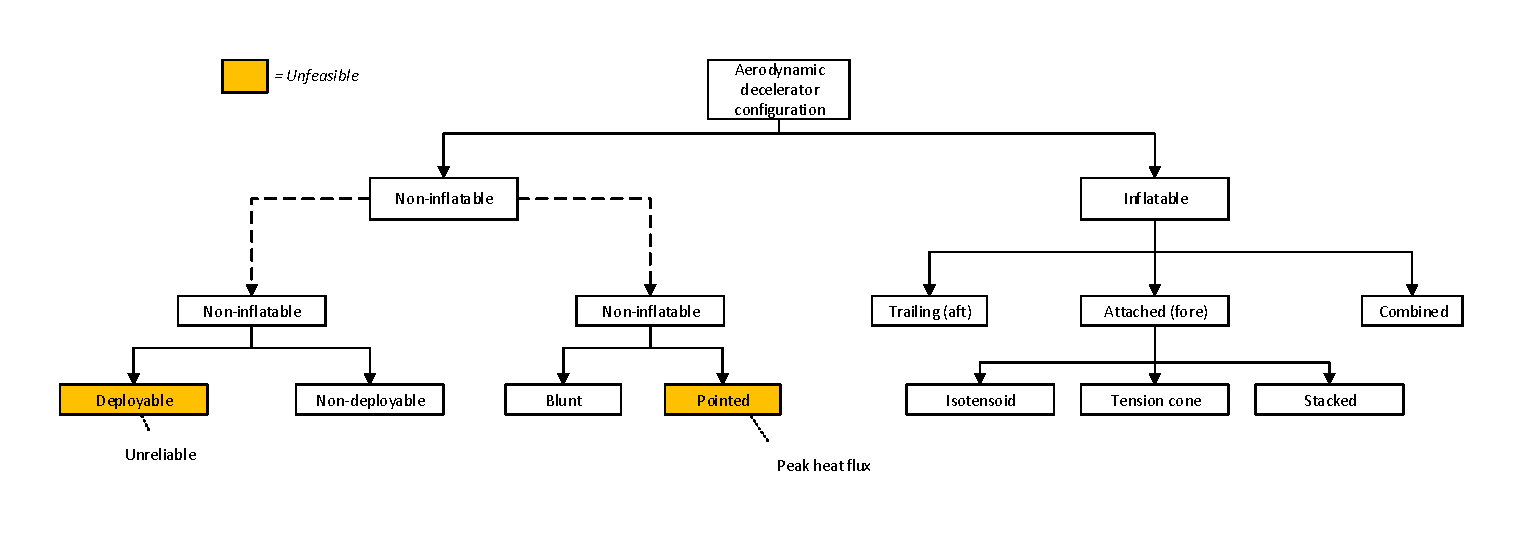
\includegraphics[width = 1.25\textwidth]{Figure/DOT_configuration.pdf}
\vspace{-5mm}
\caption{\acrlong{dot} for entry vehicle configurations}
\label{fig:dotshape}
\end{figure}

\begin{figure}[H]
\centering
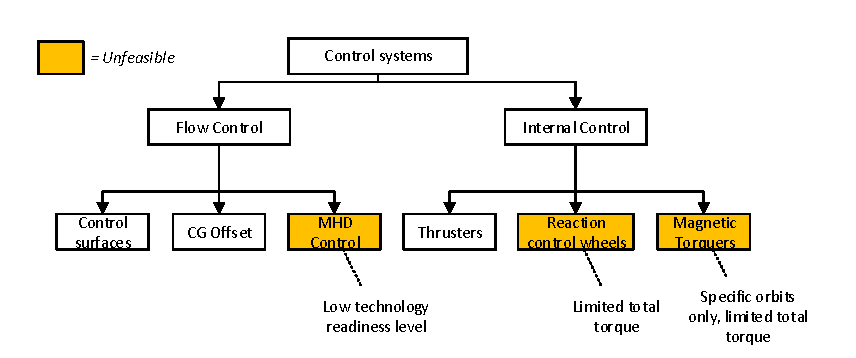
\includegraphics[width = 0.93\textwidth]{Figure/DOT_control.pdf}
\vspace{-5mm}
\caption{\acrlong{dot} for control systems}
\label{fig:dotcontrol}
\end{figure}

\begin{figure}[H]
\centering
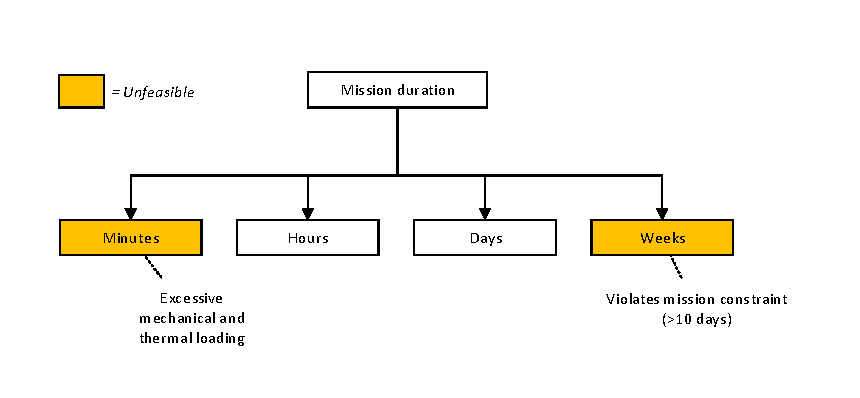
\includegraphics[width = 1.0\textwidth]{Figure/DOT_missionduration.pdf}
\vspace{-5mm}
\caption{\acrlong{dot} for mission duration}
\label{fig:dotduration}
\end{figure}

From the eighteen options yielded by combining the 6 feasible shapes and 3 feasible control systems shown in Figures \ref{fig:dotshape} and \ref{fig:dotcontrol} some may be disregarded immediately since they cannot practically be combined. For obvious reasons it is crucial that each concept configuration features at least one deemed feasible control system. From this point onward the concept shape will be considered leading. 

The control systems from Fig. \ref{fig:dotcontrol} are considered separately for each of these shapes. Due to infeasibility of exotic control concepts such as the, for now, deemed infeasible \gls{mhd} the control system can be integrated with each structure. This can be done since the control systems themselves do no longer require strict geometric properties as would be required by for example \gls{mhd} control.

Table \ref{tab:designconcepts} shows the design options that will be considered within this report. The check-marked control systems are further investigated for their feasibility and performance within section \ref{sec:ccs}. It must be noted that the control configurations of Table \ref{tab:designconcepts} feature the primary control mechanism. These may always be appended later on in the design process, after the trade-off, if additional control systems increase the overall systems performance. 

\begin{table}[H]
	\caption{Generation of design concepts}
	\label{tab:designconcepts}
	\centering
		\begin{tabular}{|p{0.3\textwidth}|p{0.14\textwidth}|p{0.14\textwidth}|p{0.14\textwidth}|} \hline 
			\textbf{Concept} & \textbf{Thrusters}	& \textbf{\gls{cg} offset} &  \textbf{Control surfaces} \\ \hline \hline
			Stacked toroid   & \cmark	& \cmark &  \cmark \\ \hline
			Isotensoid		 & \cmark	& \cmark &  \cmark\\  \hline
			Tension cone	 & \cmark	& \cmark &  \cmark \\ \hline
			Trailing ballute & \xmark	& \xmark &  \cmark \\ \hline
			Combined 		 & \xmark	& \xmark &  \cmark \\ \hline
			Rigid  		   	 & \cmark	& \cmark &  \cmark \\ \hline
		\end{tabular}
\end{table}

From Table \ref{tab:designconcepts} it can be noted that all shape configurations are deemed feasible for at least one control system. To yield a total of five system-level concepts the combined concept is disregarded. This is the case because it is considered to be too similar to a trailing ballute concept. A trailing concept will still require a heat shield in front of the capsule and can therefore be considered, in some aspects, a combined configuration as well. It is therefore considered that a deployable inflatable at the front will have no additional advantages. A small deployable structure will have a similar performance as the trailing configuration, but features the additional complexity of the front inflation system. A large inflatable located on the front of the capsule will however place the aft inflatable in its wake, making it effectively useless for producing drag. Removing the aft decelerator will however yield a "simple" stacked toroid, isotensoid or tension cone configuration, depending on the structure located on the front of the capsule. For these reasons the trailing concept will not be considered. 
 
The infeasible combinations of control systems are further detailed in \ref{sec:ccs}, together with a general description of each control system concept. 

\subsection{Concept configurations} \label{sec:conf}
In this section a the global configuration of each of the final five shapes is considered. They are sketched and described shortly in the sections below. Moreover a simple \gls{fbd} is provided for each concept to gain insight into, where applicable, the structural principle of each of the concepts.

\paragraph{Stacked toroid}

Fig. \ref{fig:conc_stacked} and \ref{fig:fbd_stacked} show the stacked toroid concept. A stacked toroid configuration features multiple inflatables which are stacked together to form the aeroshell. These inflatables are consequently covered with a thermal protection layer. In this design the payload is placed aft of the aeroshell.\

\begin{figure}[H]
\centering
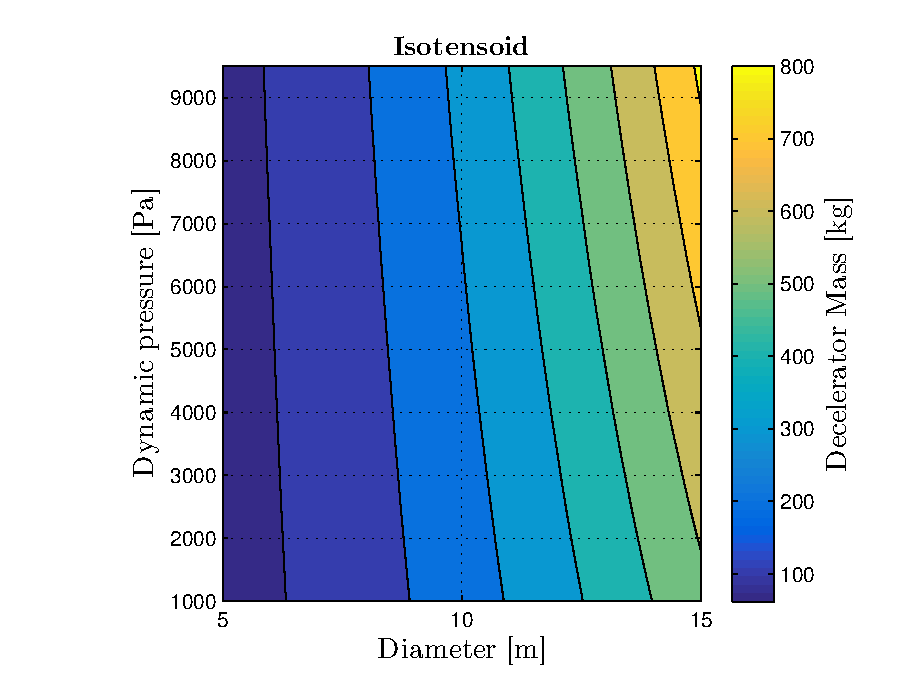
\includegraphics[width = 0.5\textwidth]{Figure/ISO_comp.eps}
\caption{A schematic view of a stacked toroid configuration}
\label{fig:conc_stacked}
\end{figure}

\begin{figure}[H]
\centering
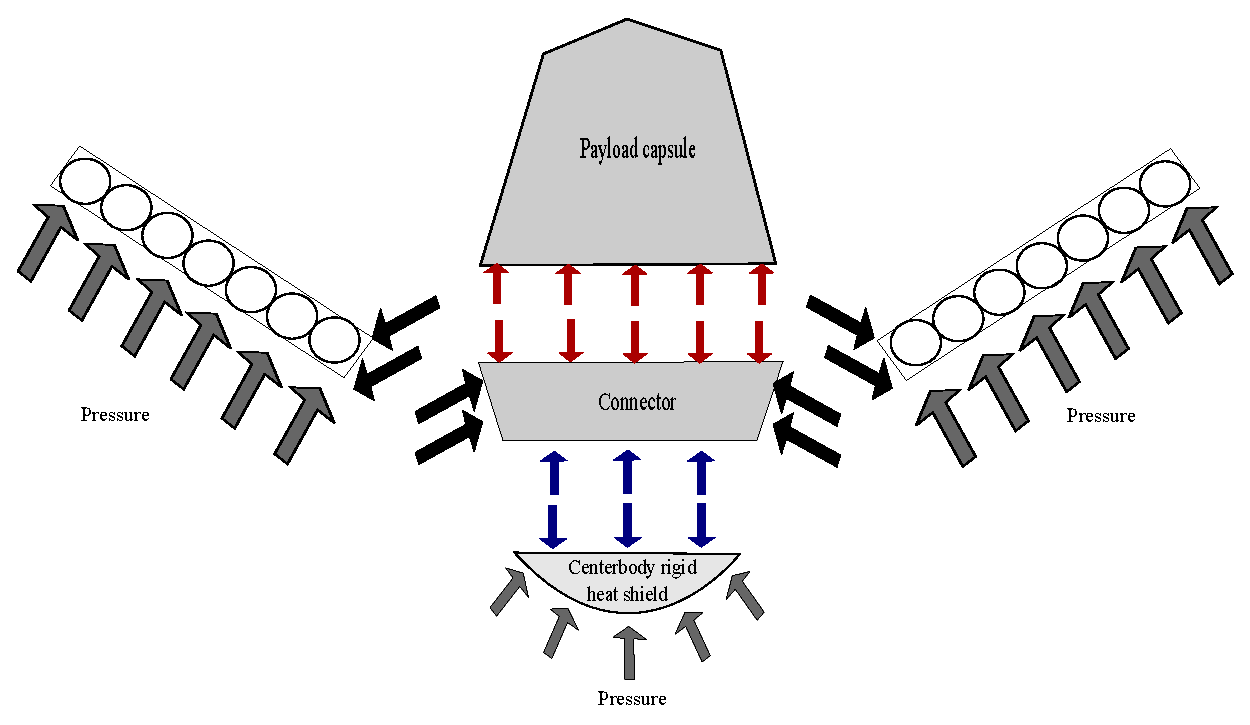
\includegraphics[width = 0.62\textwidth]{Figure/FBD_stacked.eps}
\caption{A \gls{fbd} of the stacked toroid configuration}
\label{fig:fbd_stacked}
\end{figure}


\paragraph{Isotensoid}

An isotensoid configuration as displayed in Fig. \ref{fig:conc_iso} and \ref{fig:fbd_iso} features a single inflatable. This inflatable covers the whole of the payload. This inflatable is relatively large and is typically inflated using ram-air \cite{Smith2011}. 

\begin{figure}[H]
\centering
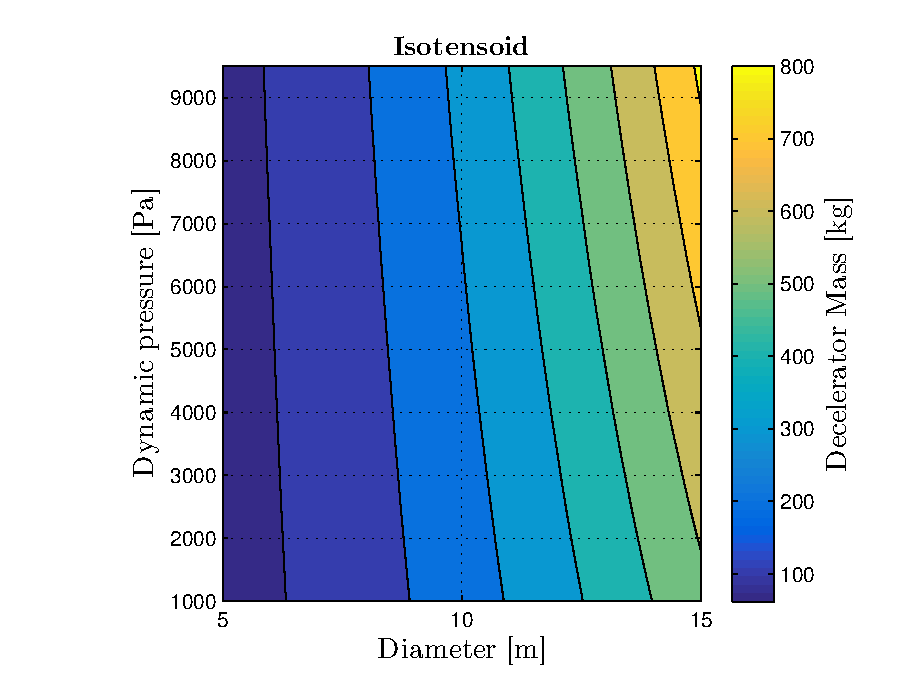
\includegraphics[width = 0.5\textwidth]{Figure/ISO_comp.eps}
\caption{A schematic view of a isotensoid configuration}
\label{fig:conc_iso}
\end{figure}

\begin{figure}[H]
\centering
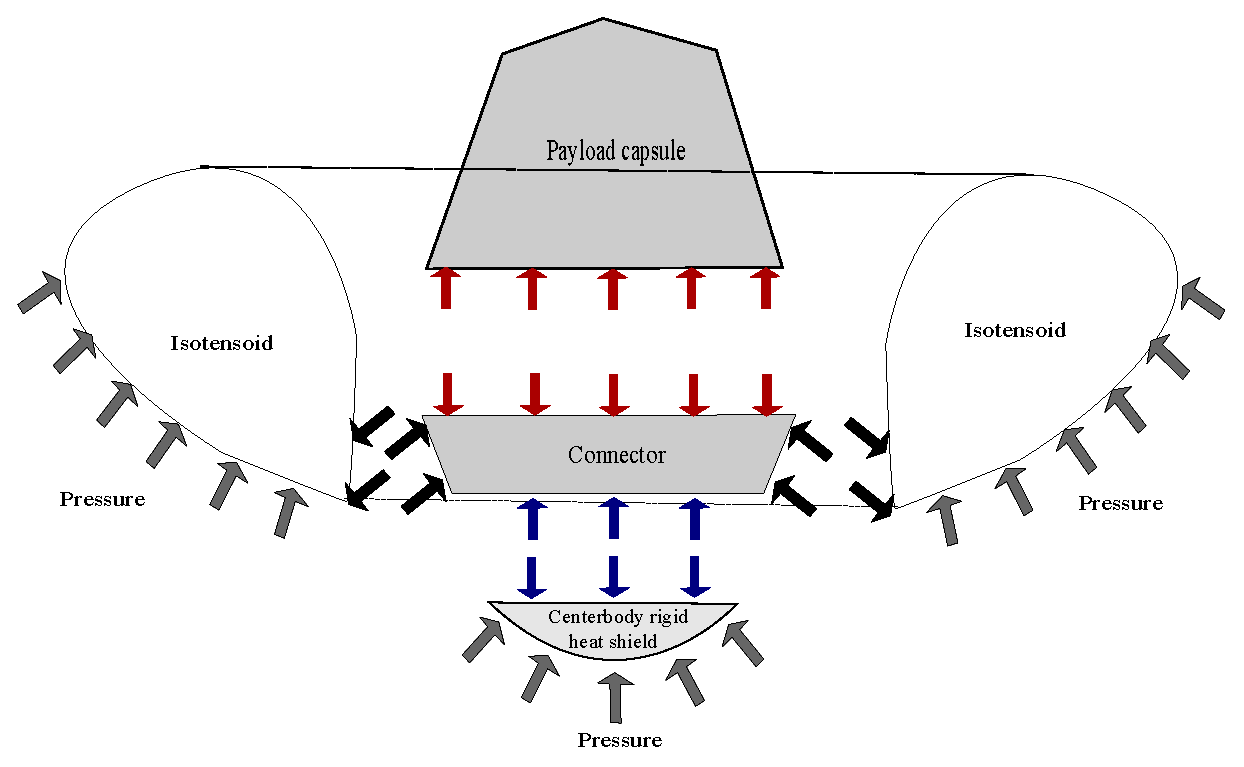
\includegraphics[width = 0.55\textwidth]{Figure/FBD_isotensoid.eps}
\caption{A \gls{fbd} of the isotensoid configuration}
\label{fig:fbd_iso}
\end{figure}

\paragraph{Tension cone}

A tension cone, as shown in Fig. \ref{fig:conc_tension} and \ref{fig:fbd_tension}  again consists only of a single inflatable. In this case the inflatable is ring formed, using the ring to provide stiffness to a web spanned within. In this configuration the aeroshell is placed front of the payload, warping around it in some extend.

\begin{figure}[H]
\centering
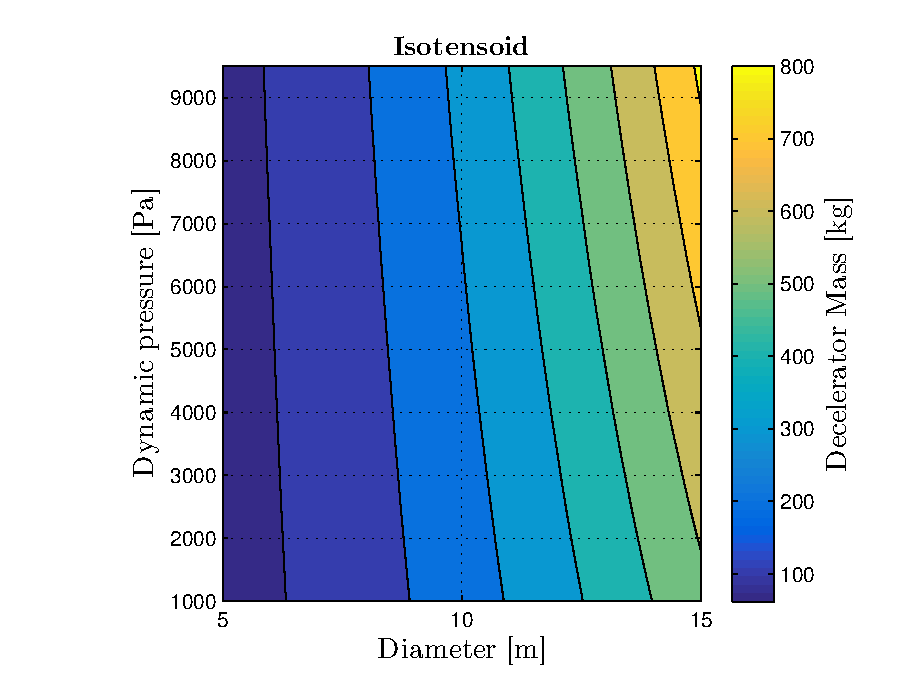
\includegraphics[width = 0.5\textwidth]{Figure/ISO_comp.eps}
\caption{A schematic view of a tension cone configuration}
\label{fig:conc_tension}
\end{figure}

\begin{figure}[H]
\centering
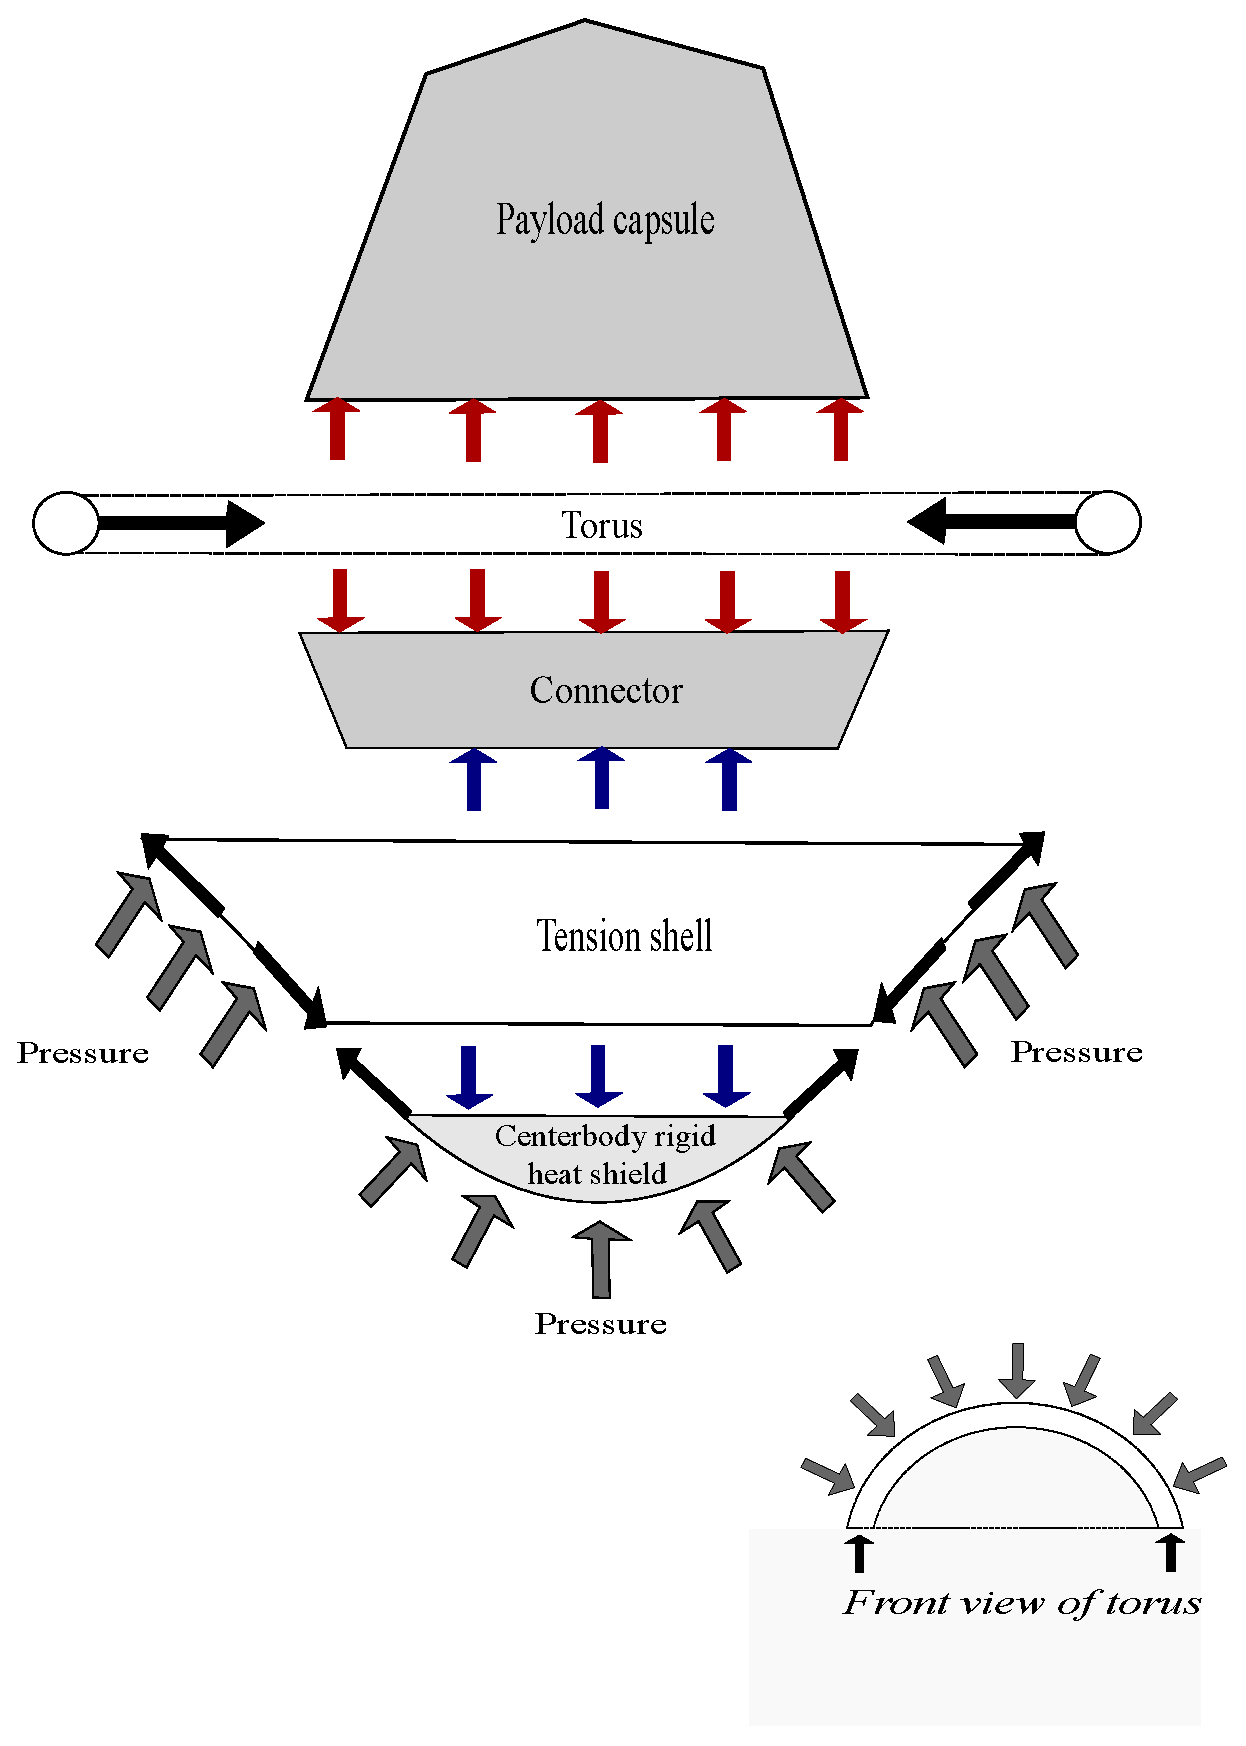
\includegraphics[width = 0.4\textwidth]{Figure/FBD_tensioncone.eps}
\caption{A \gls{fbd} of the tension cone configuration}
\label{fig:fbd_tension}
\end{figure}

\paragraph{Trailing}

Fig. \ref{fig:conc_trailing} \ref{fig:fbd_trailing} show a trailing configuration. A trailing configuration consist of two parts. An aft-placed inflatable, typically referred to as the trailing, and a front placed rigid heat shield. Since the inflatable is placed aft the payload is directly exposed to the atmosphere requiring the addition of the rigid heat shield. The shock waves induced by the front of the payload consequently create a wake aft of the payload. A typical trailing device is therefore ring formed to stay out of this wake is also displayed by Fig. \ref{fig:conc_trailing}. This is also the trailing configuration as treated within this report.

\begin{figure}[H]
\centering
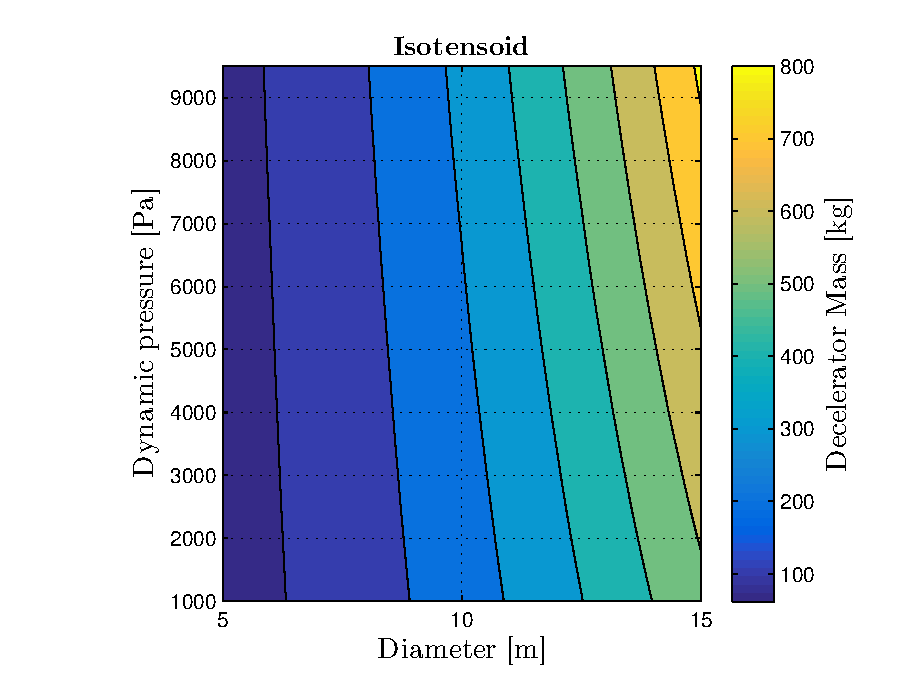
\includegraphics[width = 0.5\textwidth]{Figure/ISO_comp.eps}
\caption{A schematic view of a trailing configuration}
\label{fig:conc_trailing}
\end{figure}

\begin{figure}[H]
\centering
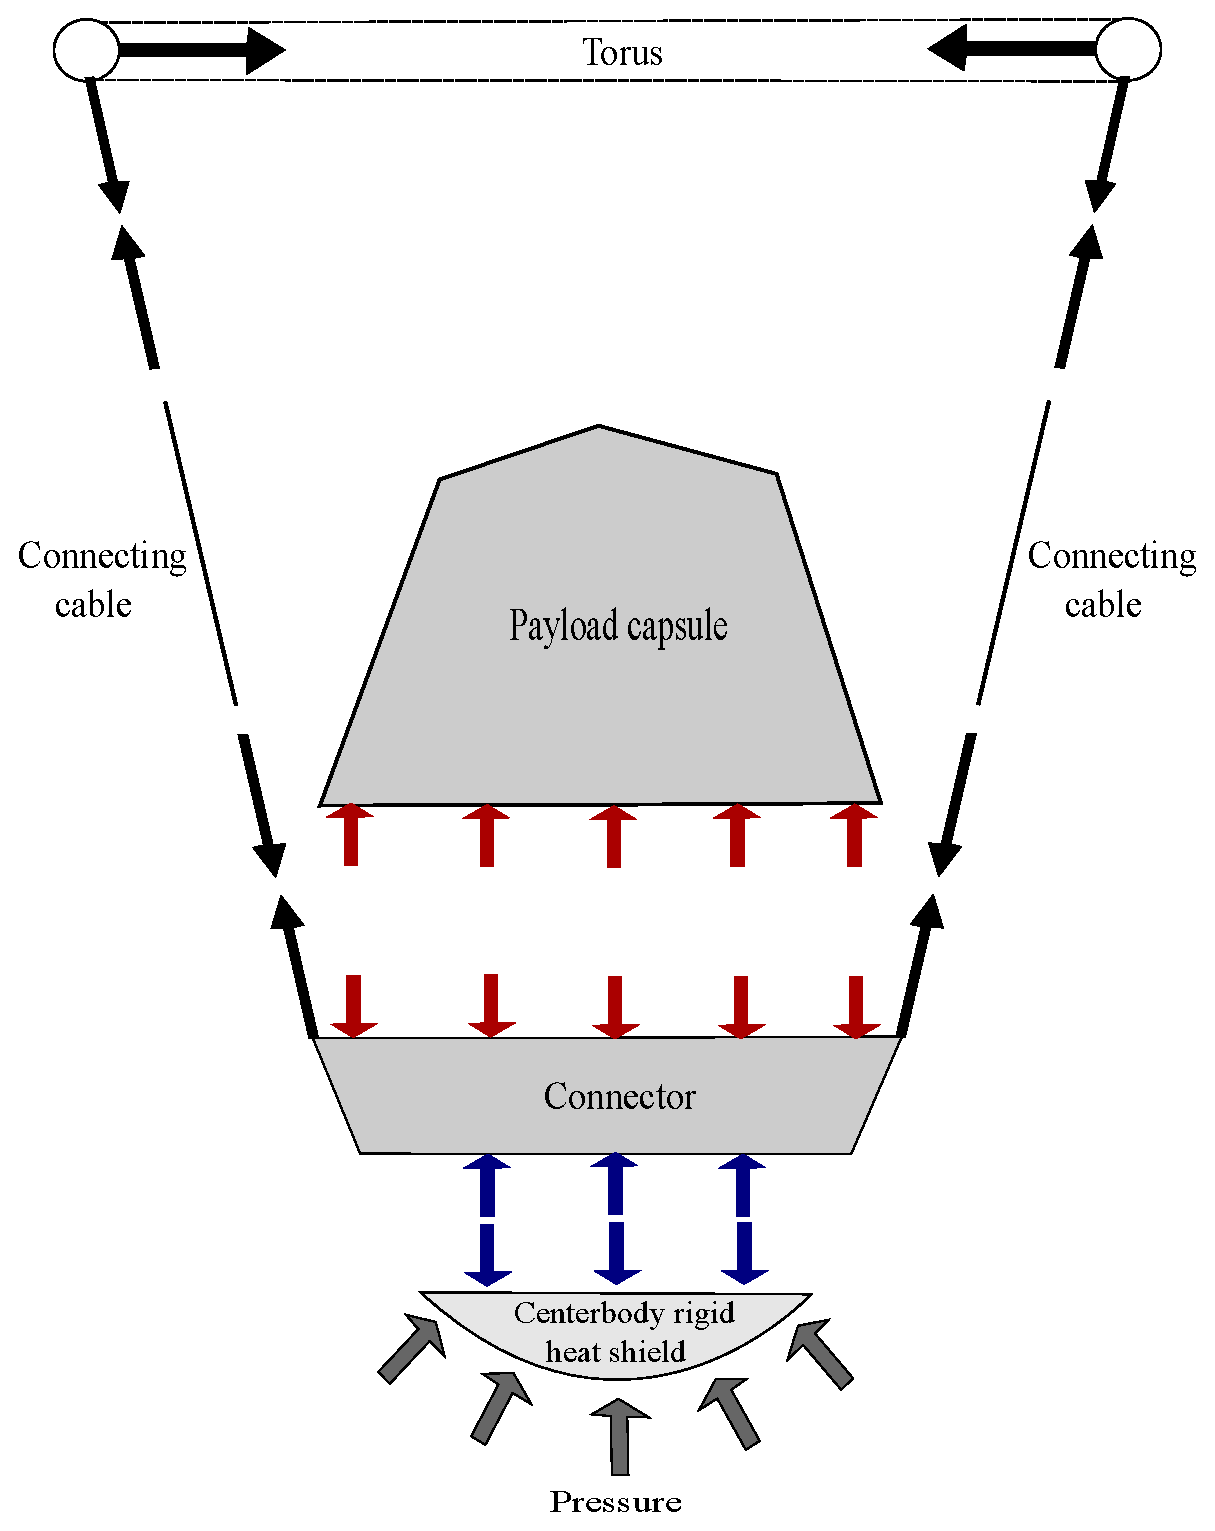
\includegraphics[width = 0.4\textwidth]{Figure/FBD_trailing.eps}
\caption{A \gls{fbd} of the trailing configuration}
\label{fig:fbd_trailing}
\end{figure}

\paragraph{Rigid}

The rigid configuration is the most typical configuration and frequently used by returns to the earth atmosphere such as in the Apollo, Soyuz or planned Orion mission. Fig. \ref{fig:conc_rigid} and \ref{fig:fbd_rigid} show the Rigid configuration. This design features a rigid heat shield in front of the payload and is the only concept featuring no inflatable parts.

\begin{figure}[H]
\centering
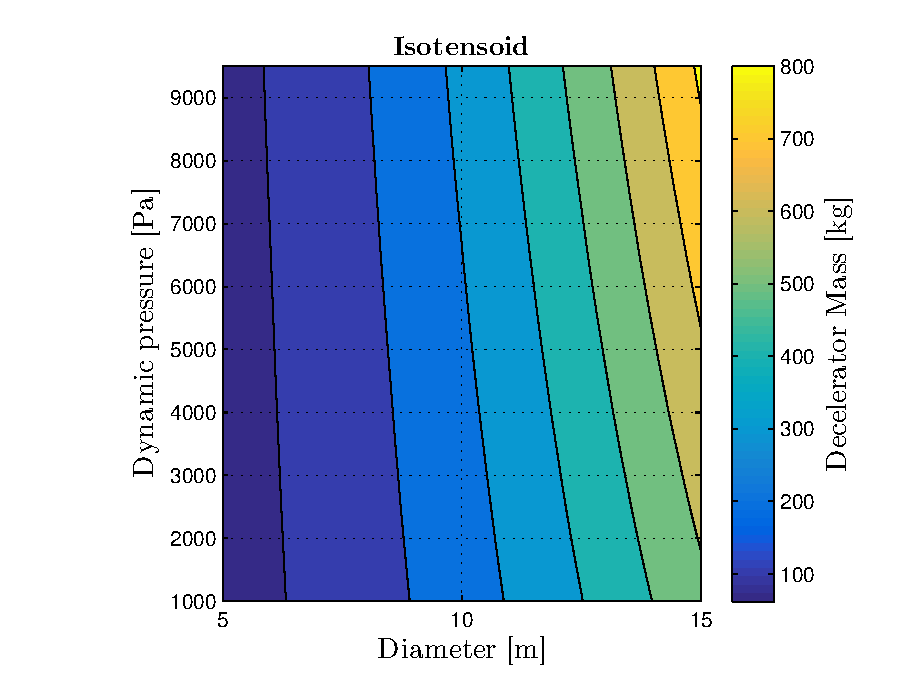
\includegraphics[width = 0.5\textwidth]{Figure/ISO_comp.eps}
\caption{A schematic view of a rigid configuration}
\label{fig:conc_rigid}
\end{figure}

\begin{figure}[H]
\centering
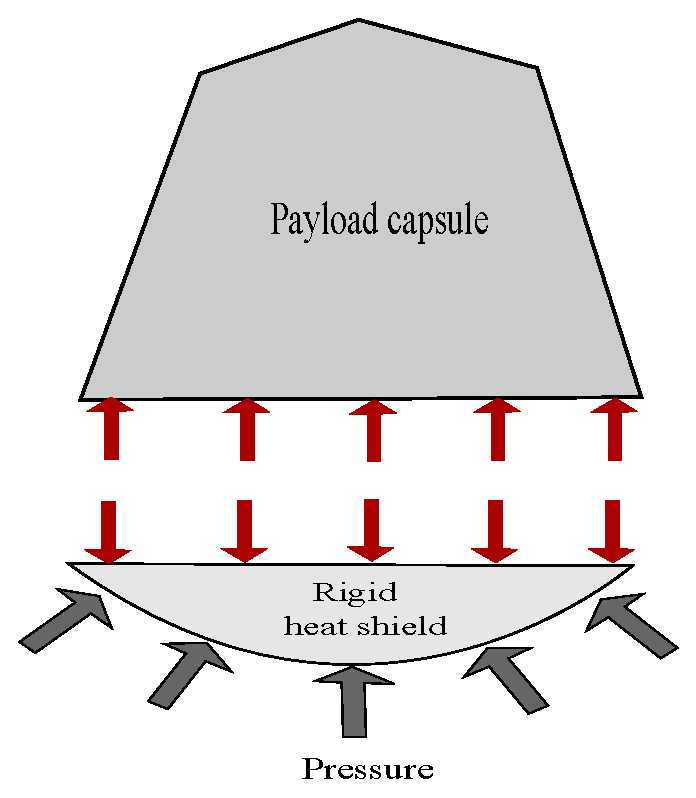
\includegraphics[width = 0.3\textwidth]{Figure/FBD_rigid.eps}
\caption{A \gls{fbd} of the rigid configuration}
\label{fig:fbd_rigid}
\end{figure}

\subsection{Concept control systems} \label{sec:ccs}
This section discusses the control systems for each of the control systems of the design option tree. This is related to the shapes of each of the concepts also serving to explain the check-marks and crosses of Table \ref{tab:designconcepts}. 

The control surfaces are not yet further detailed within the midterm report. Development risk and control system mass is however taken into account by considering the feasible control concepts and by considering the aerodynamic properties of the concepts. The latter is detailed in Chapter \ref{ch:aero_analysis}.

\subsubsection{\gls{cg} offset}
A \acrfull{cg}-offset can be used in two ways. A static \gls{cg}-offset, which is typically employed, and an actively controlled \gls{cg} offset system. The latter has already been demonstrated in the \gls{irve}-3 mission \cite{Dillman2012}. This was however considering smaller payload module mass fractions. Applying a \gls{cg} offset yields a change in the moment balance around the \gls{cg}. In a \gls{cg}-offset control system this property is actively used for the manipulation of the system. 

The use of a \gls{cg}-offset control system does however have speed limitations as changes in the location of the centre of gravity are slow.

The usage of an active \gls{cg}-offset system for the trailing and combined configurations was not deemed feasible due to the existence of aft elements which are connected to the capsule through a non-rigid connection, such as a cable. Thus, for the trailing concept active \gls{cg}-offset control was not deemed feasible.

\subsubsection{Thrusters}
Thrusters are the only internal control system that was deemed feasible and will hence always be featured on the spacecraft. For the part of the mission up to the first entry into the Martian atmosphere thrusters will thus be used in any case. Thrusters can however also be employed as a primary control surface, which obviously increases the mass and usage of the systems.

Thrusters are deployed in pairs for the control of the spacecraft, such that they can deliver a torque couple. The amount of torque delivered is a linear function of the relative distance between the thrusters and is constrained for this design by launcher constraints. 

In terms of development risk thrusters are frequently used and feature minimal risk.

Thrusters are not considered for the trailing and combined configuration. Due to the aft elements of these designs thruster cannot be considered as the primary control mechanism. Due to the large moments of inertia (due to aft elements) and very high stability of the aft systems (e.g. compare to a parachute) thrusters cannot be considered due their inefficiency. 

\subsubsection{Control surfaces}
Control surfaces have been subdivided into two forms; body flaps and morphing of the whole structure, which are both covered below.

\paragraph{Body flaps}
A control system with body flaps features deployable surfaces to manipulate the flow around the spacecraft. Body flaps have previously been deployed at for example the Space Shuttle missions. It must however be noted that its usage was limited to supersonic Mach numbers at higher atmospheric densities. As such it is a possible control concept for the rigid structure.

Body flaps on inflatable structures have not yet been featured and are not deemed feasible. This is the case because when a body flap is placed on the outer extremity of an inflatable surface said surface will deflect due to the forces exerted by the flap. Thus the combination of body flaps and inflatable structures is not deemed to be feasible. The usage of body flaps for the Mach numbers considered would also incur a significant development risk.

\paragraph{Morphing}
In morphing concepts the external shape of the aeroshell is manipulated in order to control the spacecraft. The difference between morphing structures and body flaps is that in a morphing structure the moving section is an integral part of the aeroshell, whereas a body flap is an additional, separate section specifically designed to be actuated. Using a morphing structure as control system is not possible in conjunction with a rigid structure, since the stiffness of the structure would require extreme control forces and thus a heavy control system. For inflatable structures (who typically have less stiffness than a rigid structure) morphing is deemed possible with exception of the isotensoid design and has already been investigated in recent years \cite{Hughes2011}.

Morphing a trailing ballute configuration would be done via the payload-ballute connection much like a parachute, where the length of the connection elements would be individually altered to change the orientation of the trailing element with respect to the flow.

In terms of development risk morphing structures are mostly at a very early conceptual phase posing significant development risks. Theoretical investigations for morphing of a stacked toroid configuration have been conducted \cite{Green2013} but no actual testing is done. One can see how employing a morphing structure as control system would thus increase the overall development risk.